% Batang di Kiri, Daun di Kanan: Diagram Batang-Daun dengan TikZ
% Dokumen LaTeX utuh, siap dikompilasi (butuh paket tikz).
% Data: 30 nilai ulangan susulan kelas 8D, sudah diurutkan:
% 42, 47, 51, 55, 58, 60, 63, 64, 67, 69, 71, 72, 74, 75, 76, 78,
% 80, 81, 83, 84, 85, 87, 88, 90, 91, 93, 94, 96, 97, 99.
% Batang = puluhan, daun = satuan. Jarak antar daun 0,55 cm.
% Median = (76 + 78) / 2 = 77 (dua daun emas pada batang 7).
\documentclass{article}
\usepackage{tikz}

\begin{document}

\section*{Diagram batang-daun: 30 nilai kelas 8D}

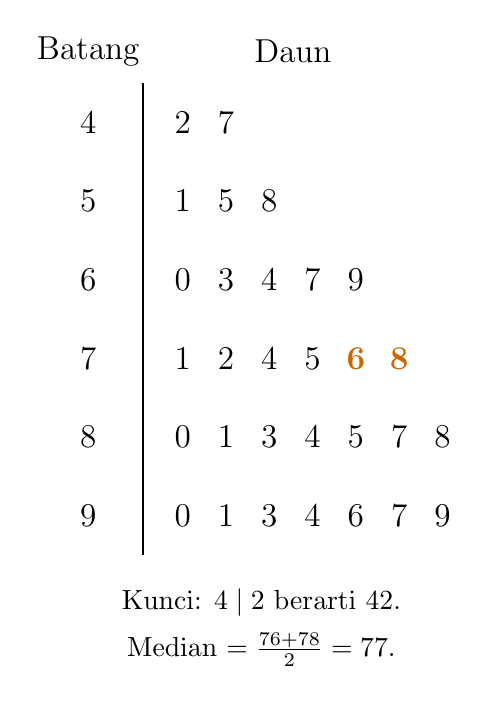
\begin{tikzpicture}[font=\large]
  % Judul kolom
  \node at (0,5.9) {Batang};
  \node at (2.6,5.9) {Daun};
  % Garis pemisah batang-daun
  \draw[thick] (0.7,5.5) -- (0.7,-0.5);
  % Baris 4: daun 2 7
  \node at (0,5) {4};
  \foreach \i/\d in {0/2, 1/7}
    \node at ({1.2 + \i*0.55},5) {\d};
  % Baris 5: daun 1 5 8
  \node at (0,4) {5};
  \foreach \i/\d in {0/1, 1/5, 2/8}
    \node at ({1.2 + \i*0.55},4) {\d};
  % Baris 6: daun 0 3 4 7 9
  \node at (0,3) {6};
  \foreach \i/\d in {0/0, 1/3, 2/4, 3/7, 4/9}
    \node at ({1.2 + \i*0.55},3) {\d};
  % Baris 7: daun 1 2 4 5 6 8 (median: 6 dan 8 diwarnai emas)
  \node at (0,2) {7};
  \foreach \i/\d in {0/1, 1/2, 2/4, 3/5}
    \node at ({1.2 + \i*0.55},2) {\d};
  \node[text=orange!80!black, font=\large\bfseries] at (3.4,2) {6};
  \node[text=orange!80!black, font=\large\bfseries] at (3.95,2) {8};
  % Baris 8: daun 0 1 3 4 5 7 8
  \node at (0,1) {8};
  \foreach \i/\d in {0/0, 1/1, 2/3, 3/4, 4/5, 5/7, 6/8}
    \node at ({1.2 + \i*0.55},1) {\d};
  % Baris 9: daun 0 1 3 4 6 7 9
  \node at (0,0) {9};
  \foreach \i/\d in {0/0, 1/1, 2/3, 3/4, 4/6, 5/7, 6/9}
    \node at ({1.2 + \i*0.55},0) {\d};
  % Kunci baca
  \node[font=\normalsize] at (2.2,-1.1) {Kunci: $4 \mid 2$ berarti $42$.};
  \node[font=\normalsize] at (2.2,-1.7) {Median $= \frac{76 + 78}{2} = 77$.};
\end{tikzpicture}

\end{document}
